% !TEX root = ../../1-te.tex
\label{musterstudienplan}
\iftoggle{winter}{
	\begin{center}
		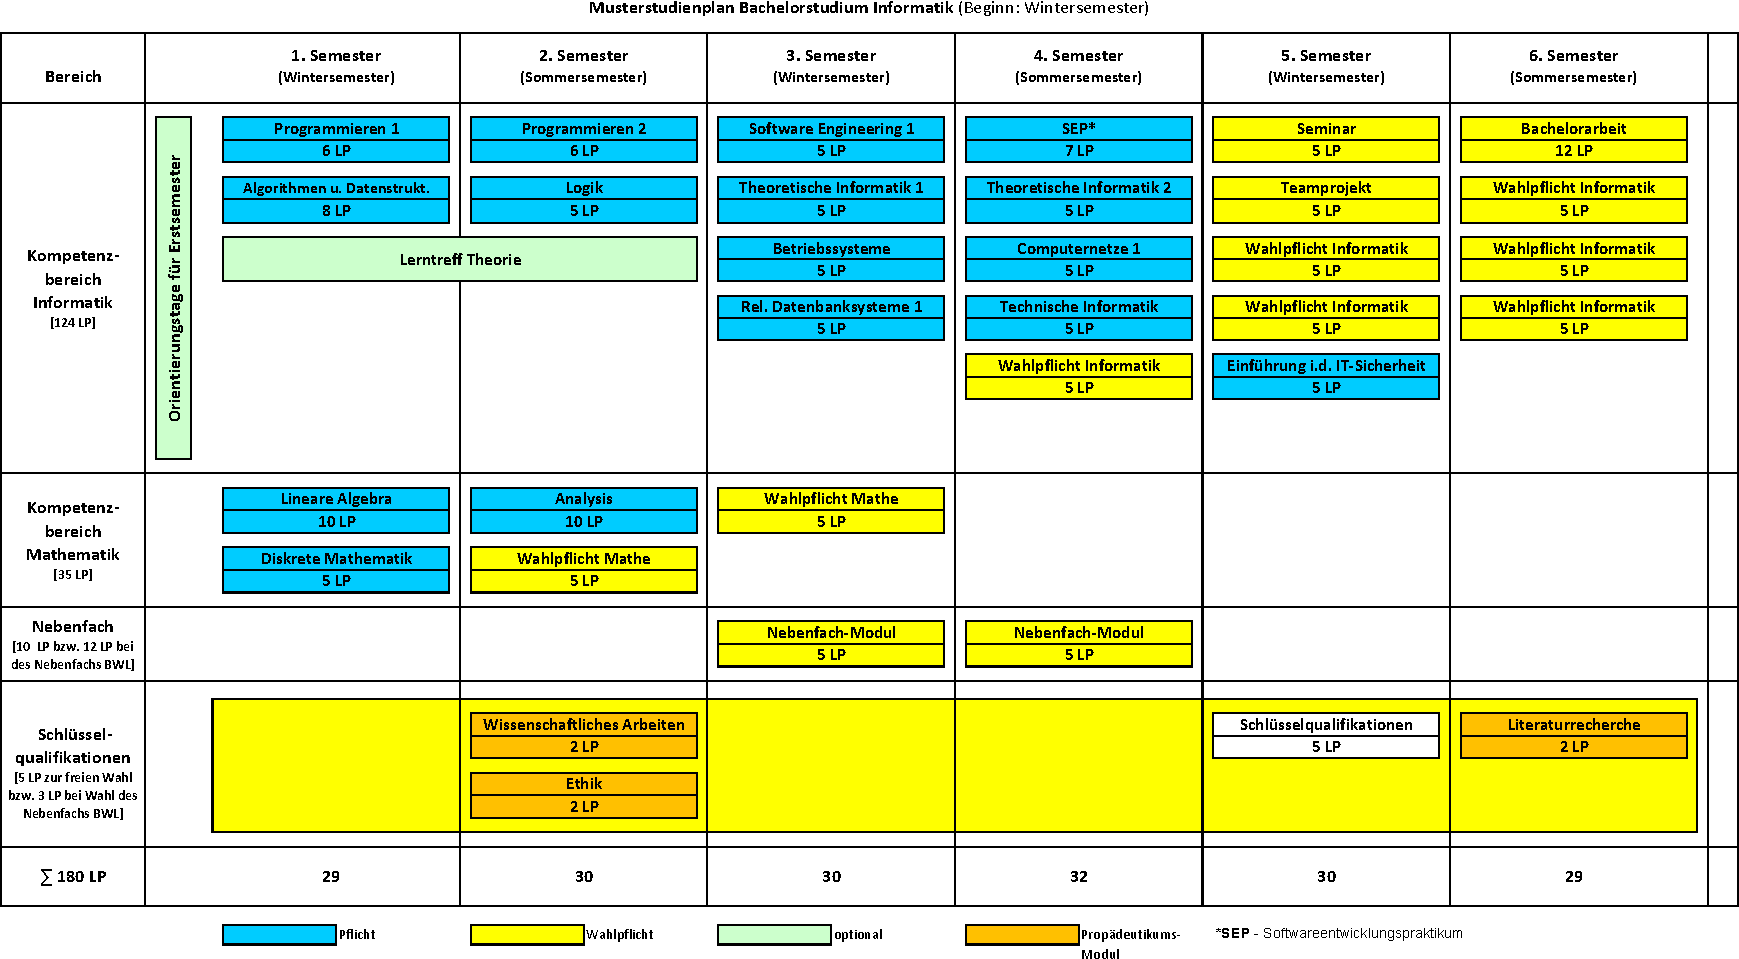
\includegraphics[angle=90, height=\textheight]{bilder/studienplan_bsc/WS-Fak.pdf}
	\end{center}

	\newpage

	\begin{center} 
		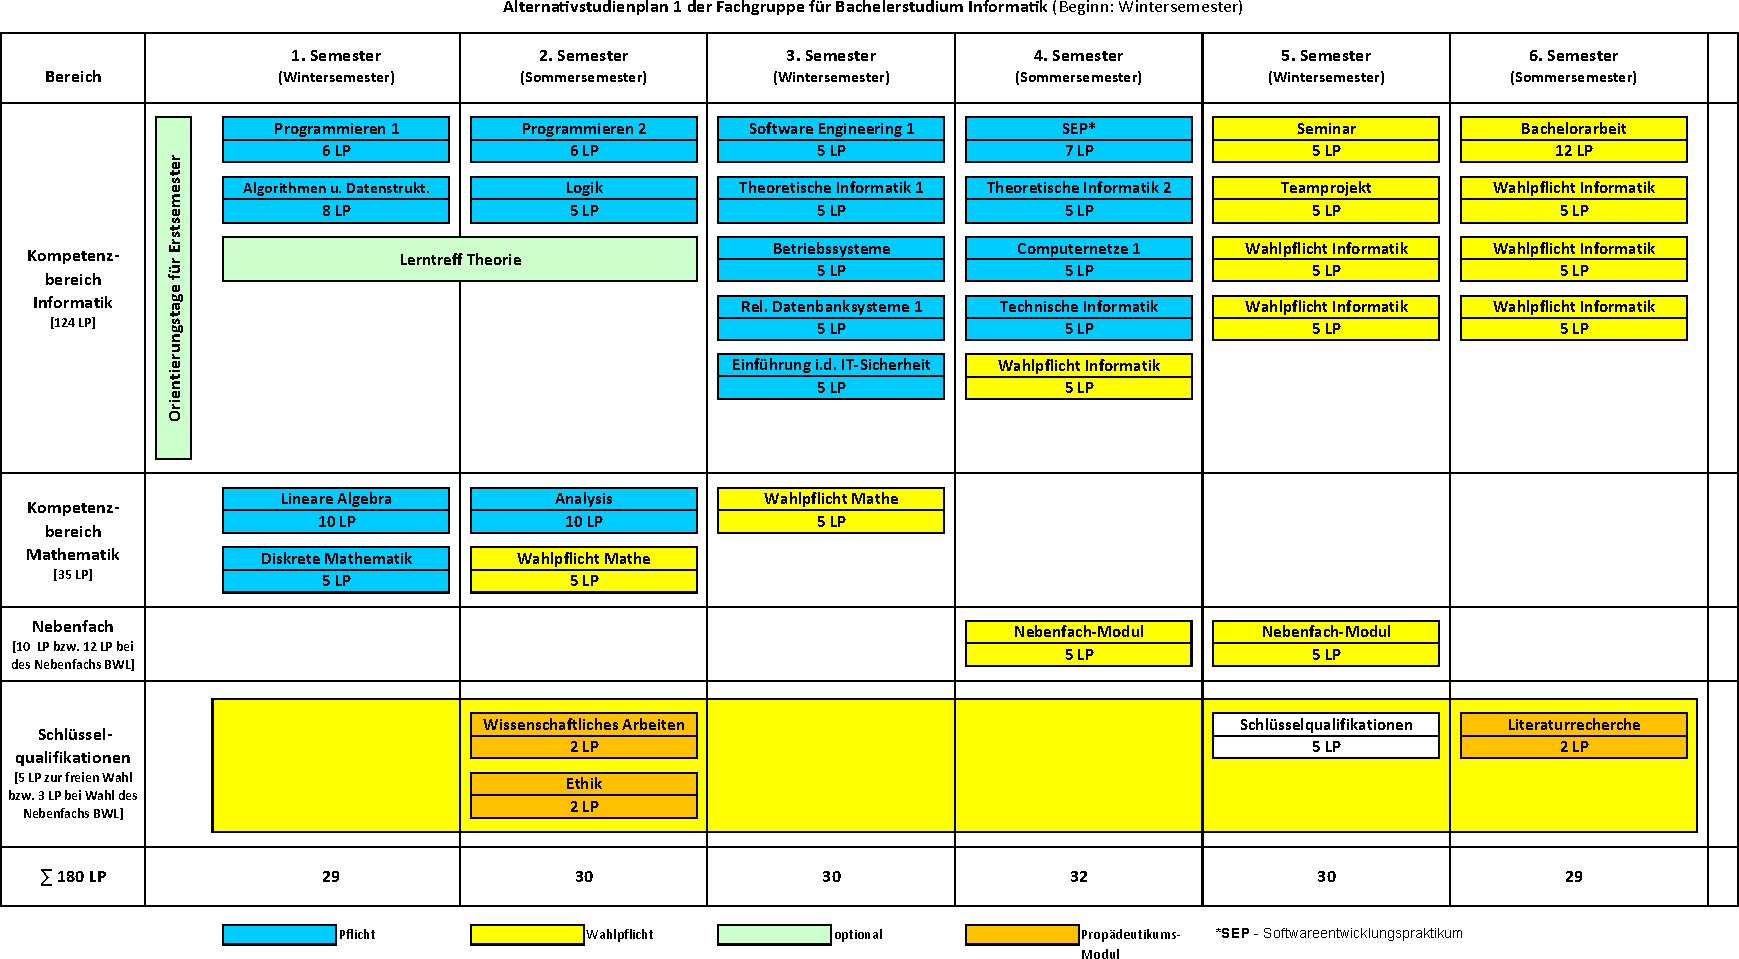
\includegraphics[angle=90, height=\textheight]{bilder/studienplan_bsc/WS-FG-easy.pdf}
	\end{center}

	\newpage

	\begin{center} 
		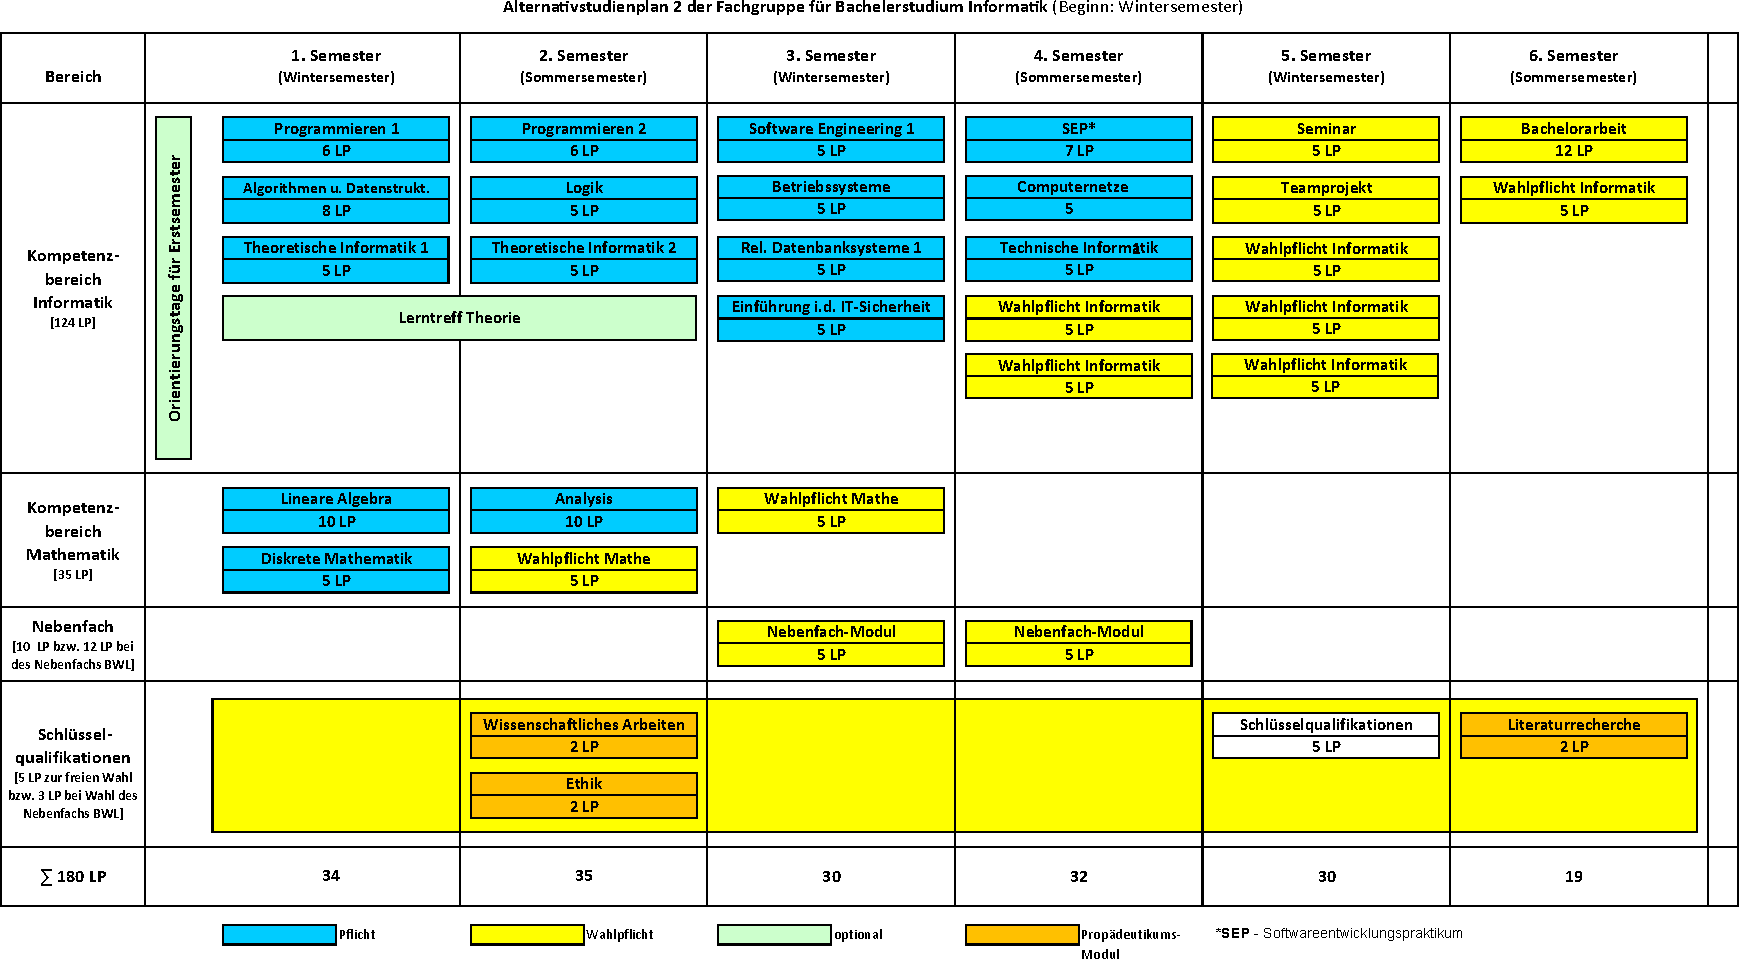
\includegraphics[angle=90, height=\textheight]{bilder/studienplan_bsc/WS-FG-hard.pdf}
	\end{center}
}{
	\begin{center}
		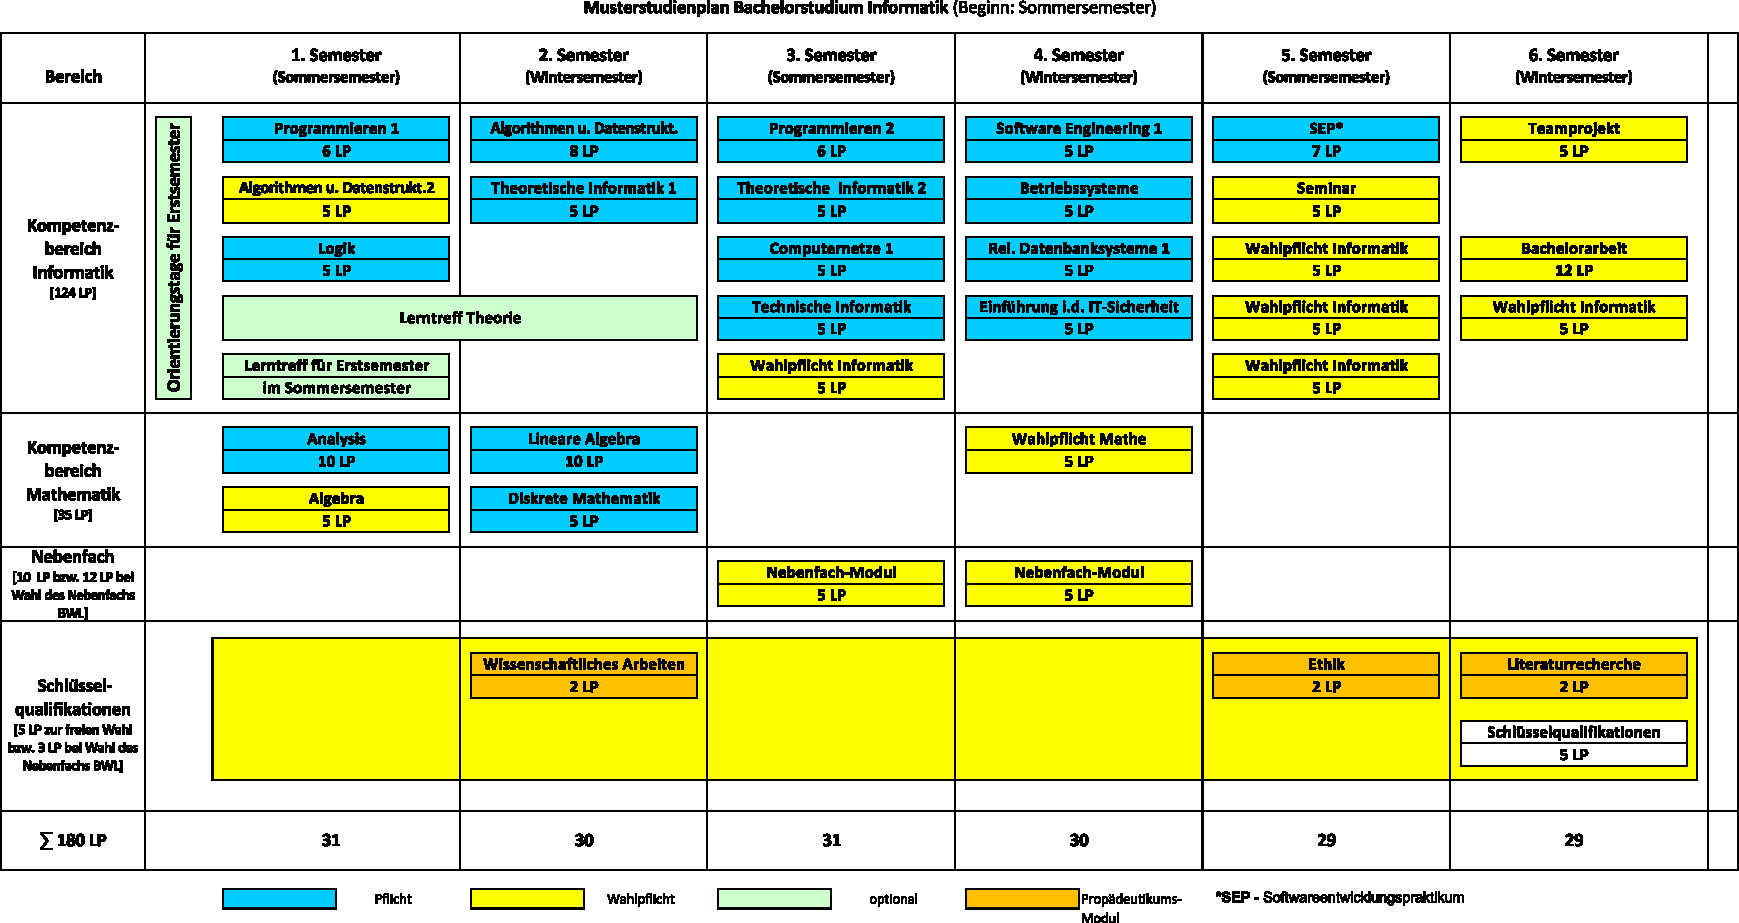
\includegraphics[angle=90, height=\textheight]{bilder/studienplan_bsc/SS-Fak.pdf}
	\end{center}

	\newpage

	\begin{center}
		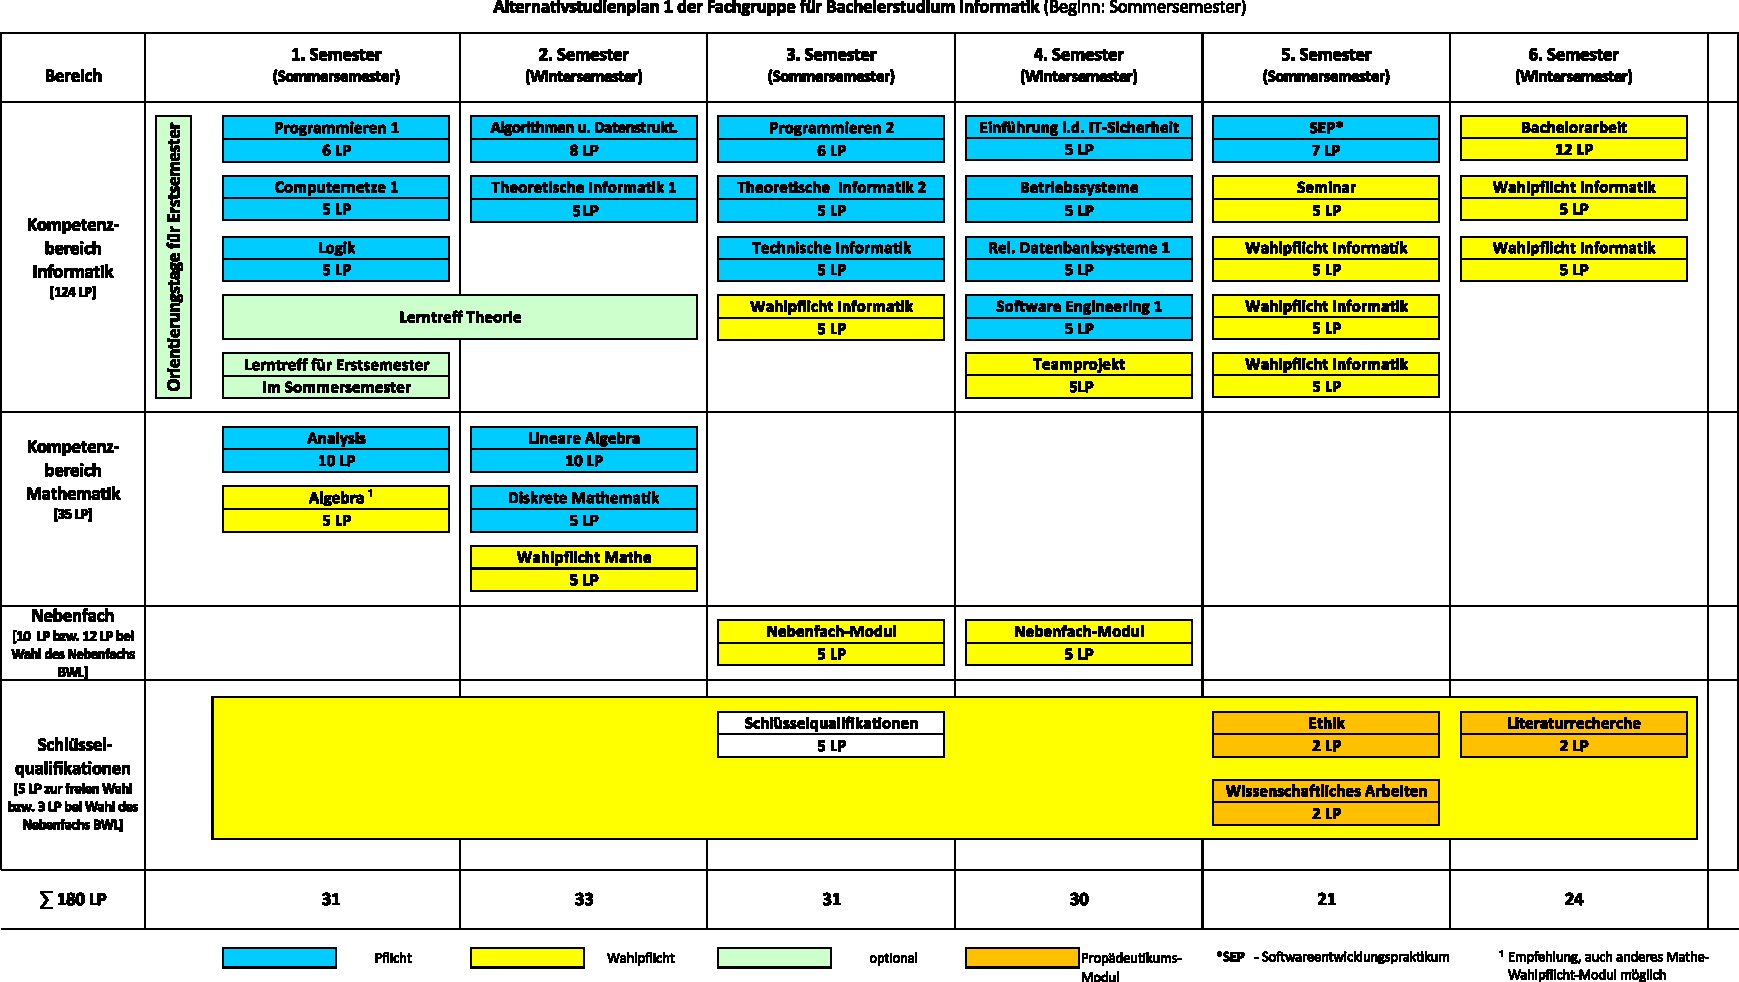
\includegraphics[angle=90, height=\textheight]{bilder/studienplan_bsc/SS-FG-david.pdf}
	\end{center}

	\newpage
	
	\begin{center}
		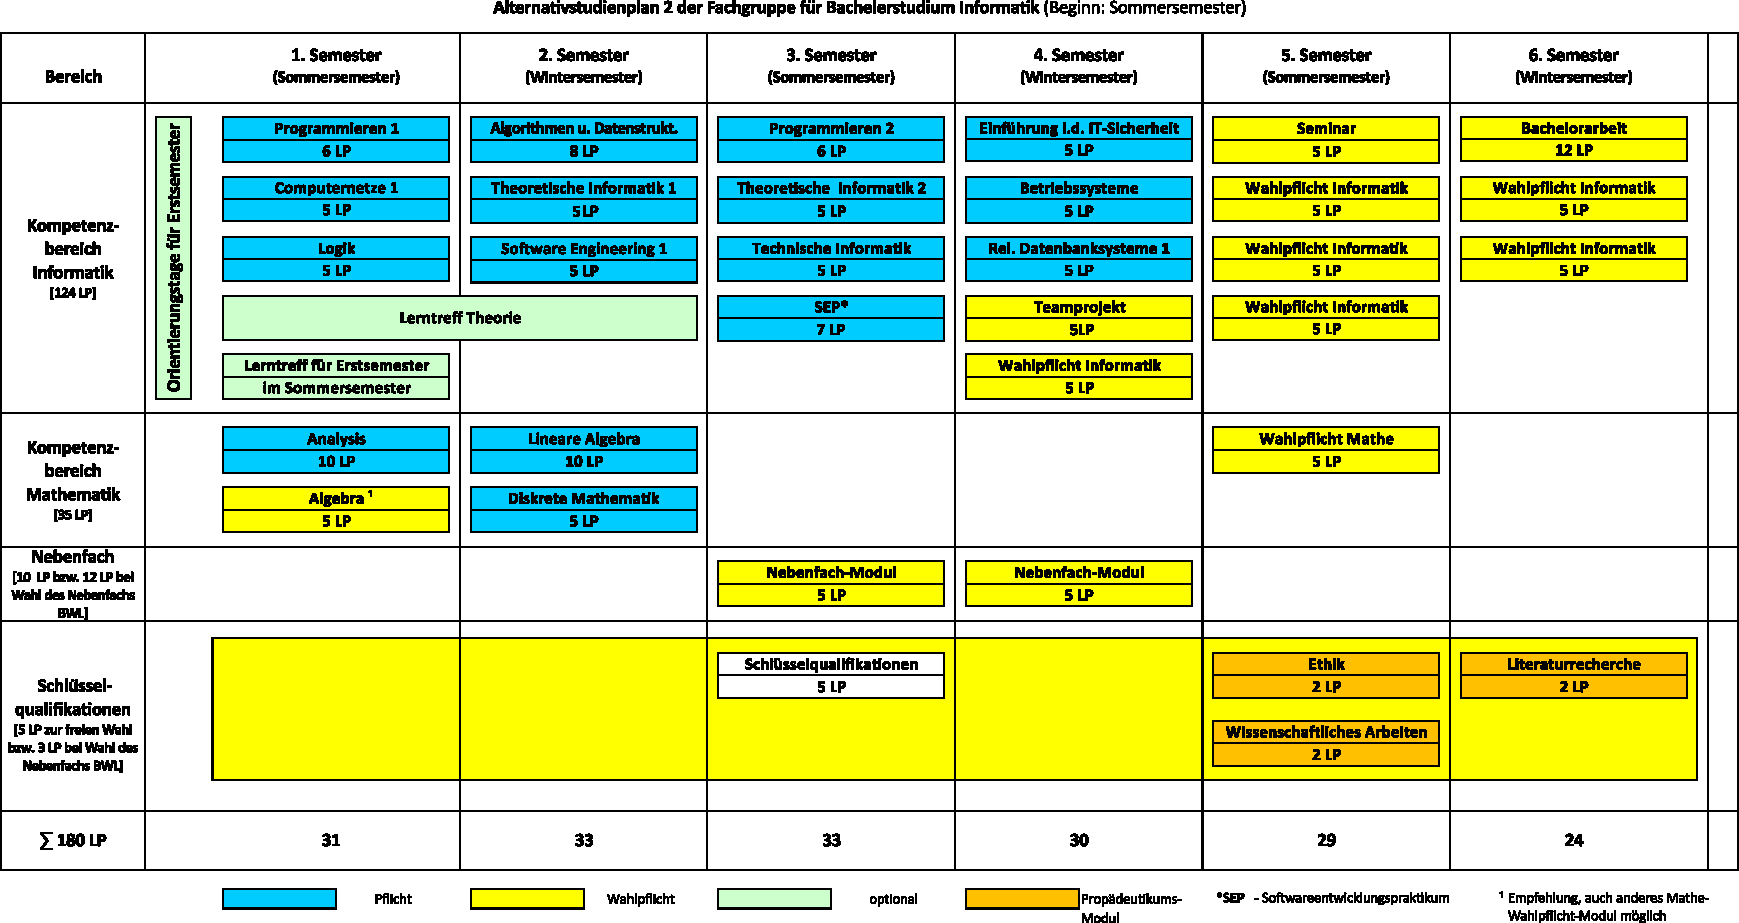
\includegraphics[angle=90, height=\textheight]{bilder/studienplan_bsc/SS-FG-hard.pdf}
	\end{center}

	\newpage
}
